\section{A new classification} \label{sec:Serotype_Classification}

\begin{figure}[!hbt]
    \centering
    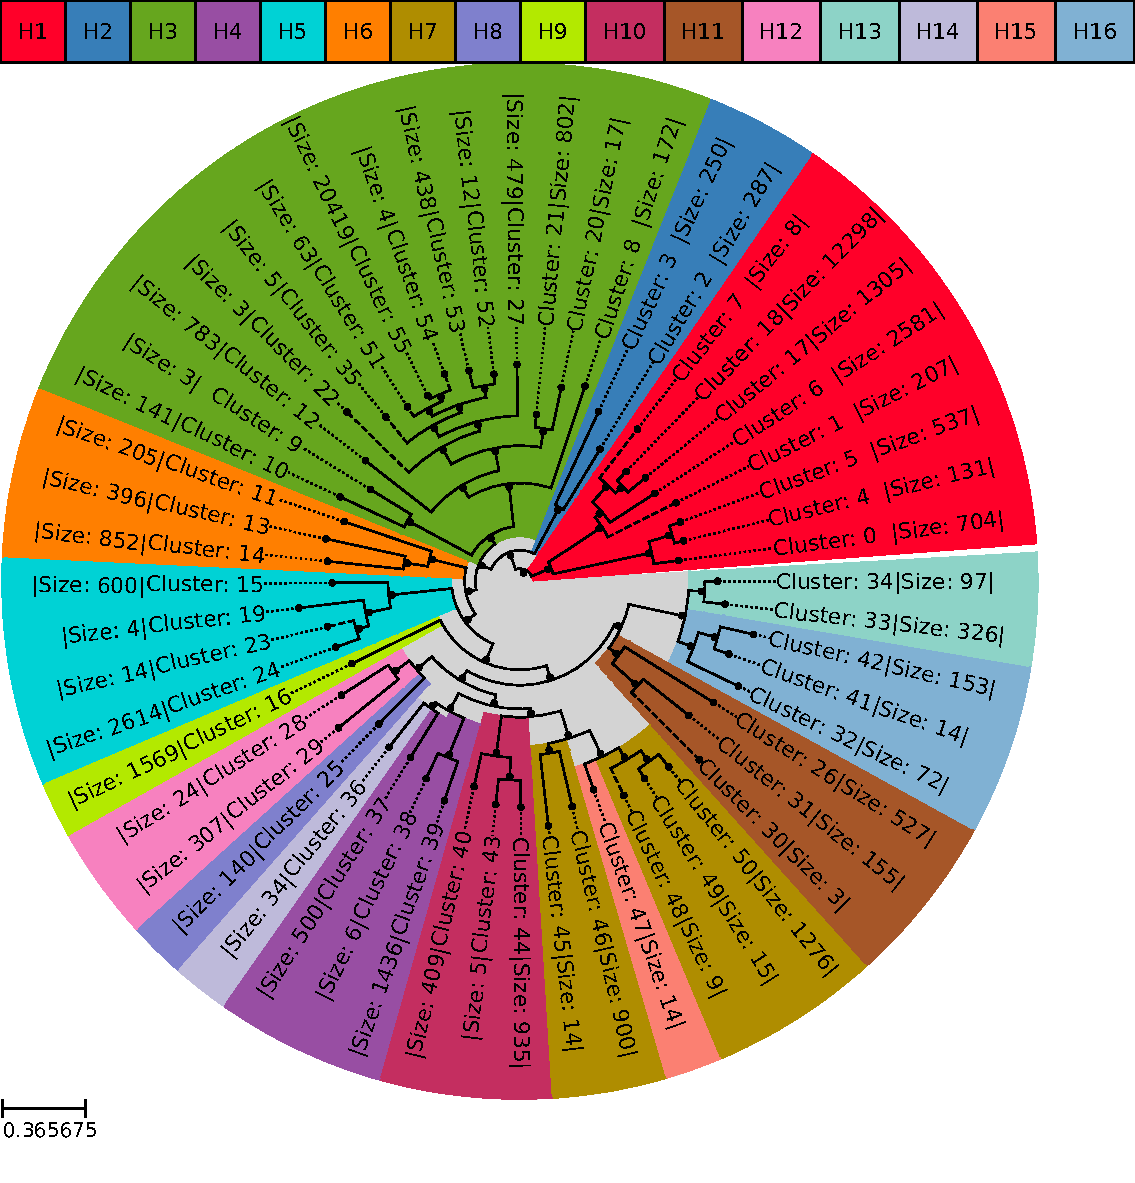
\includegraphics[width=\textwidth]{Results/Clustertree_Segment_4.pdf}
    \caption[Clustering tree of segment 4]{\textbf{Clustering tree of segment 4.} The cluster tree of segment 4 clustering, using the combination of \texttt{PCA} and the Kneedle Algorithm (PK) with a reduction to 50 instead of 30 dimensions (\autoref{fig:PCA_Cluster_Knee_4}). The labeling of the clusters in the tree is based on the subtype of the contained sequences. Unclassified sequences of a cluster are reclassified as a given subtype if sequences of only this subtype are present in the cluster in addition to the unclassified ones. Unlabeled clusters contain sequences from at least two subtypes and zero or more unclassified sequences. Dotted lines in the tree indicate the same host.}
    \label{fig:Result_Clustertree_Segment_4}
\end{figure}

Reannotation of the most likely false annotated sequence in \autoref{fig:PCA_Clusteree_Knee_4} \textbf{\textsf{C}} as well as increasing of the components in \texttt{PCA} successfully raised the accuracy of the pipeline. Thus, the clustering was performed according to the PK method, that proved to give the most stable results, with 50 components reduction instead of 30. Clustering errors found in the previous section were resolved successfully as H13 and H16 are now completely divided, with the mentioned small but still present difference between these subtypes. Also, all clusters of H3 are now present in direct connection to each other and no cluster not homogeneous for one subtype exist anymore.

\vspace{1em}
%neue classification vorschlagen blablabla
% vielleicht bisschen evolution black sea gull etc

Resulting from this improved clustering of segment 4 a new classification involving 57 groups instead of 18 subtypes is proposed (\autoref{fig:Result_Clustertree_Segment_4}). By pairwise comparison of random 10 sequence samples of these groups the similarity inside these groups is described in \autoref{fig:Proof_Clustertree_Segment_4}. To avoid creating a bias, the result for accidental comparisons of sequences with the same accession are ignored and not considered in calculations of respective mean values. Samples of 10 sequences were used due to the high amount of computational power that is necessary for this calculation. For segment 4 calculation involves $10^2$ pairwise alignments, for every of the 57 clusters to each other. Making $57^2\cdot 10^2$ calculations.

\begin{figure}[!hbt]
    \centering
    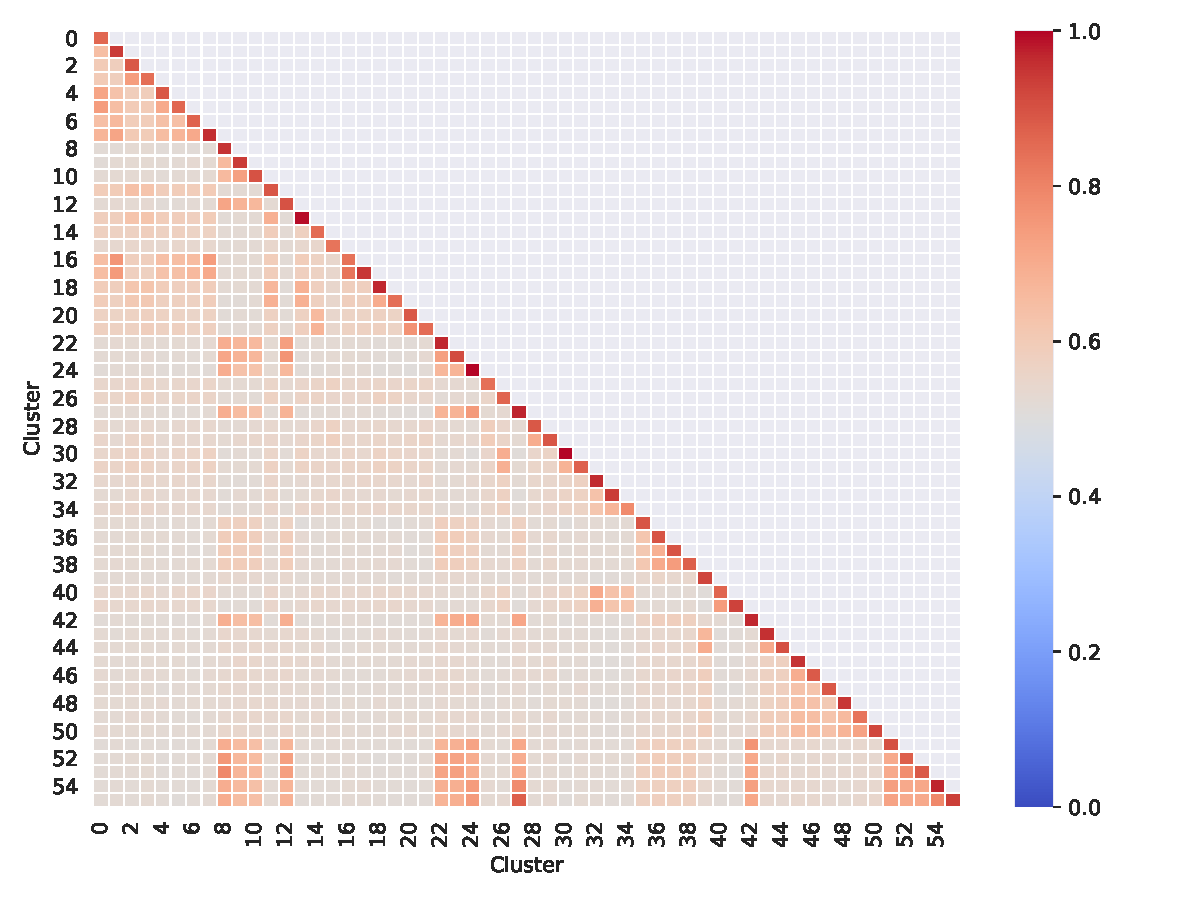
\includegraphics[width=\textwidth]{Results/Cluster_Difference_Segment_4.pdf}
    \caption[Similarity matrix of segment 4 clusters]{\textbf{Similarity matrix of segment 4 clusters.}. Random samples of up to 10 sequences of every cluster in \autoref{fig:Result_Clustertree_Segment_4} were compared by pairwise alignments with the samples of all other clusters. Less than 10 sequences were only used in clusters containing less than 10 sequences. The percentage of similarity was calculated for very alignment making a matrix of up to $10\times10$ holding the similarity values of the samples comparisons. The mean of the matrix was then calculated and written as the given cluster interactions mean similarity. This was repeated for every possible cluster interaction resulting in the presented figure. Interactions of the same clusters were reduced to only different sequences, results of alignments with sequences having the same accession were removed, thereby, preventing bias creation. The mean of these up to 100 comparisons for every cluster interaction are colored according to their similarity from 1.0 or 100\% similarity in red to 0.0 or 0\% similarity in blue.}
    \label{fig:Proof_Clustertree_Segment_4}
\end{figure}

All clusters in \autoref{fig:Proof_Clustertree_Segment_4} have the highest similarities with themselves and mostly high similarities with clusters of the same subtype. For instance cluster 0, share some degree of sequence identity with other clusters stemming from the same subtype H1, as shown in \autoref{fig:Proof_Clustertree_Segment_4}. However, the highest similarity of around 90\% is only shared with other sequences of the cluster itself, which makes this cluster very self contained. 

\vspace{1em}

Exceptions for the relative high similarity to other clusters of the same subtypes are the subtypes H7 and H15 with the clusters 45 to 50, as well as H4 and H14 with clusters 35 to 38. There was no clear separation performed as the clusters merge with other subtypes in higher tree nodes, although other clusters of the same subtype are still available (\autoref{fig:Result_Clustertree_Segment_4}). The similarities of these cluster, are also high compared to the other subtype and indicate a relation neglected by the current subtype classification. The almost uniform H7 subtree of clusters 45, 46, 48, 49, and 50 is divided by the one and only cluster of subtype H15 cluster 47. When comparing the sequence similarities in \autoref{fig:Proof_Clustertree_Segment_4}, the highest similarity persist inside the clusters themselves, but the cross similarities of cluster 45 and 46 to 47, 48, 49, and 50 are around 65\% without big difference between subtype H7 and H15. Further pointing to more subtle but present differences between and inside of the current subtypes. 

\vspace{1em}

With this pipeline blueprint created by adjusting the clustering for segment 4 in the previous sections, all \gls{IAV} segments could be clustered the same way, since no subtype information is necessary for the clustering. Subtype labeling of the tree was performed as guideline and was the only part involving actual sequence position to subtype evaluation. Thereby, the clustering trees for other segments, except segment 6, are unlabeled. All other cluster trees and similarity matrix graphics, as well as tables containing sequence cluster assignment and the tables containing the values used to create the graphics are presented in the \autoref{chap:Appendix}. Hereby new classifications for all segments based on $k$-mer frequency vectors are proposed, containing 28 groups for segment 1, 28 for segment 2, 29 for segment 3, the shown 57 for segment 4, 26 for segment 5, 40 for segment 6, 30 for segment 7 and 24 groups for segment 8 \autoref{tab:Result_Cluster}. 

\vspace{1em}

The groups of the segments 1 to 3, 5, 7, and 8 share by far more overall similarity, therefore, less clusters were created (\autoref{chap:Appendix}). Still, the similarity inside the clusters themselves is higher than the cross similarity and, thereby, solid clustering by the proposed clustering method was possible despite the overall higher similarity. Higher similarity of the segments not encoding the surface protein is most likely reasoned by the lower evolutionary pressure. The higher pressure of the surface proteins is necessary to ensure infection of the host cells. 

\vspace{1em}

While the clusters of segment 4 seem to be very self contained and give a good representation on possible subdivisions inside the subtypes, the trees based on evolutionary distances increase the subtypes distance even more (\autoref{fig:PCA_Guidetree_Centroid_4} and \autoref{fig:Simple_Clustertree_MSA}). Present day research propose a phylogenic tree of \gls{IAV} that is split in four subtrees \autocite{wei_next-generation_2020}. The subdivisions are mostly present in the clustering tree in \autoref{fig:Result_Clustertree_Segment_4}. Still, there are some difference primarily the higher-ranking structure of the subtypes. In \textcite{wei_next-generation_2020} subtype H3 is contained in a subtree alongside H4 and H14 and H9 in a subtree with H8 and H12. This relations are not present in \autoref{fig:Result_Clustertree_Segment_4}. Though, other subtrees contain subtypes similar to the proposed phylogenic tree in \textcite{wei_next-generation_2020}. Aside from that, the order of the subtrees in \autoref{fig:Result_Clustertree_Segment_4} do not match the one from the pyhlogenic tree.

\begin{figure}[!hbt]
    \centering
    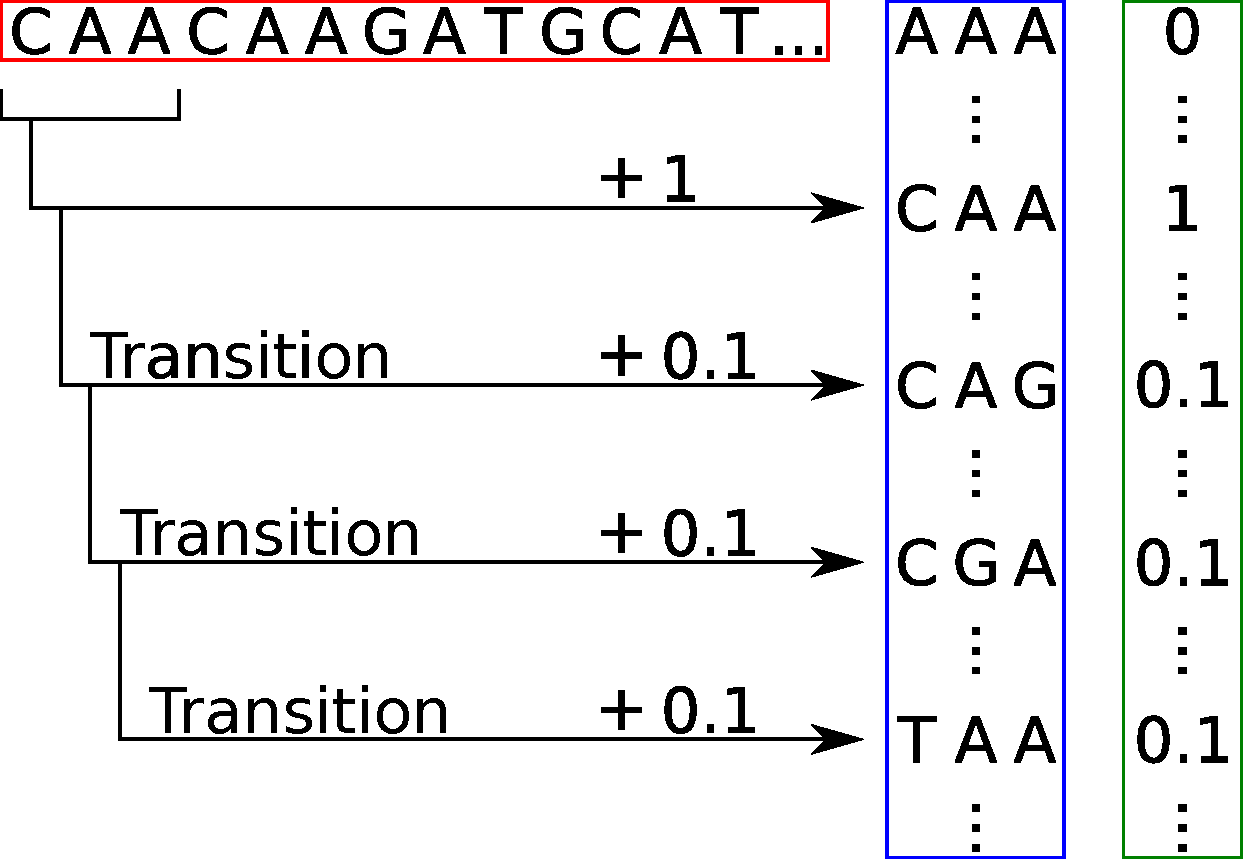
\includegraphics[width=0.5\textwidth]{Graphics/Transition.pdf}
    \caption[7-mer vector calculation involving transitions]{\textbf{7-mer vector calculation involving transitions.} An example genomic sequence (red box) is splitted into 3-mers. The sequences 3-mers are then compared to the list of all $4^3$ possible 3-mer constellations (blue box) Based on the occurrence number of the lists 3-mers in the sequence a vector with $4^3$ components is created (green box).}
    \label{fig:trans}
\end{figure}

As already mentioned the proposed method for \gls{IAV} clustering did not acknowledge evolutionary distances. Transitions and transversion for example are handled as nucleotide differences without a higher or lower chance of change. When including mutation chances in the $k$-mer frequency clustering, the relation of whole subtypes subtrees might improve and give a result more similar to the one proposed in \textcite{wei_next-generation_2020}. Because \texttt{HDBCSCAN} only uses existing distance metrics, when not using the precalculated option, which should be avoided at any case, the $k$-mer frequency vectors themselves have to be change in some way. Therefore, \autoref{fig:trans} illustrate a possible option for inclusion of evolution inside $k$-mer frequency vectors, by considering all mutations of a given $k$-mer with low representation value. Vectors containing $k$-mers only apart with single mutations are, thus, closer to each other in the high-dimensional vector space. The magnitude of these values have to be considered wisely and should be subject of future research optimizing the proposed clustering even more.